% !TEX root = ../../main.tex

\section{HarmonyOS 移动端核心模块实现}

HarmonyOS 移动端是普通用户使用系统的主要入口，主要实现登录认证、首页入口、手语资源浏览、手势训练、实时识别、句子视频识别和个人中心等功能。
移动端实现的重点是将后端资源数据、Python 实时识别能力和句子视频识别结果组织为用户可操作的页面流程，使用户能够顺利完成从资源选择到训练反馈的完整操作。

移动端核心页面效果如图~\ref{fig:chapter05-mobile-core-ui} 所示。

\begin{figure}[H]
  \centering

  \begin{subfigure}[t]{0.235\textwidth}
    \centering
    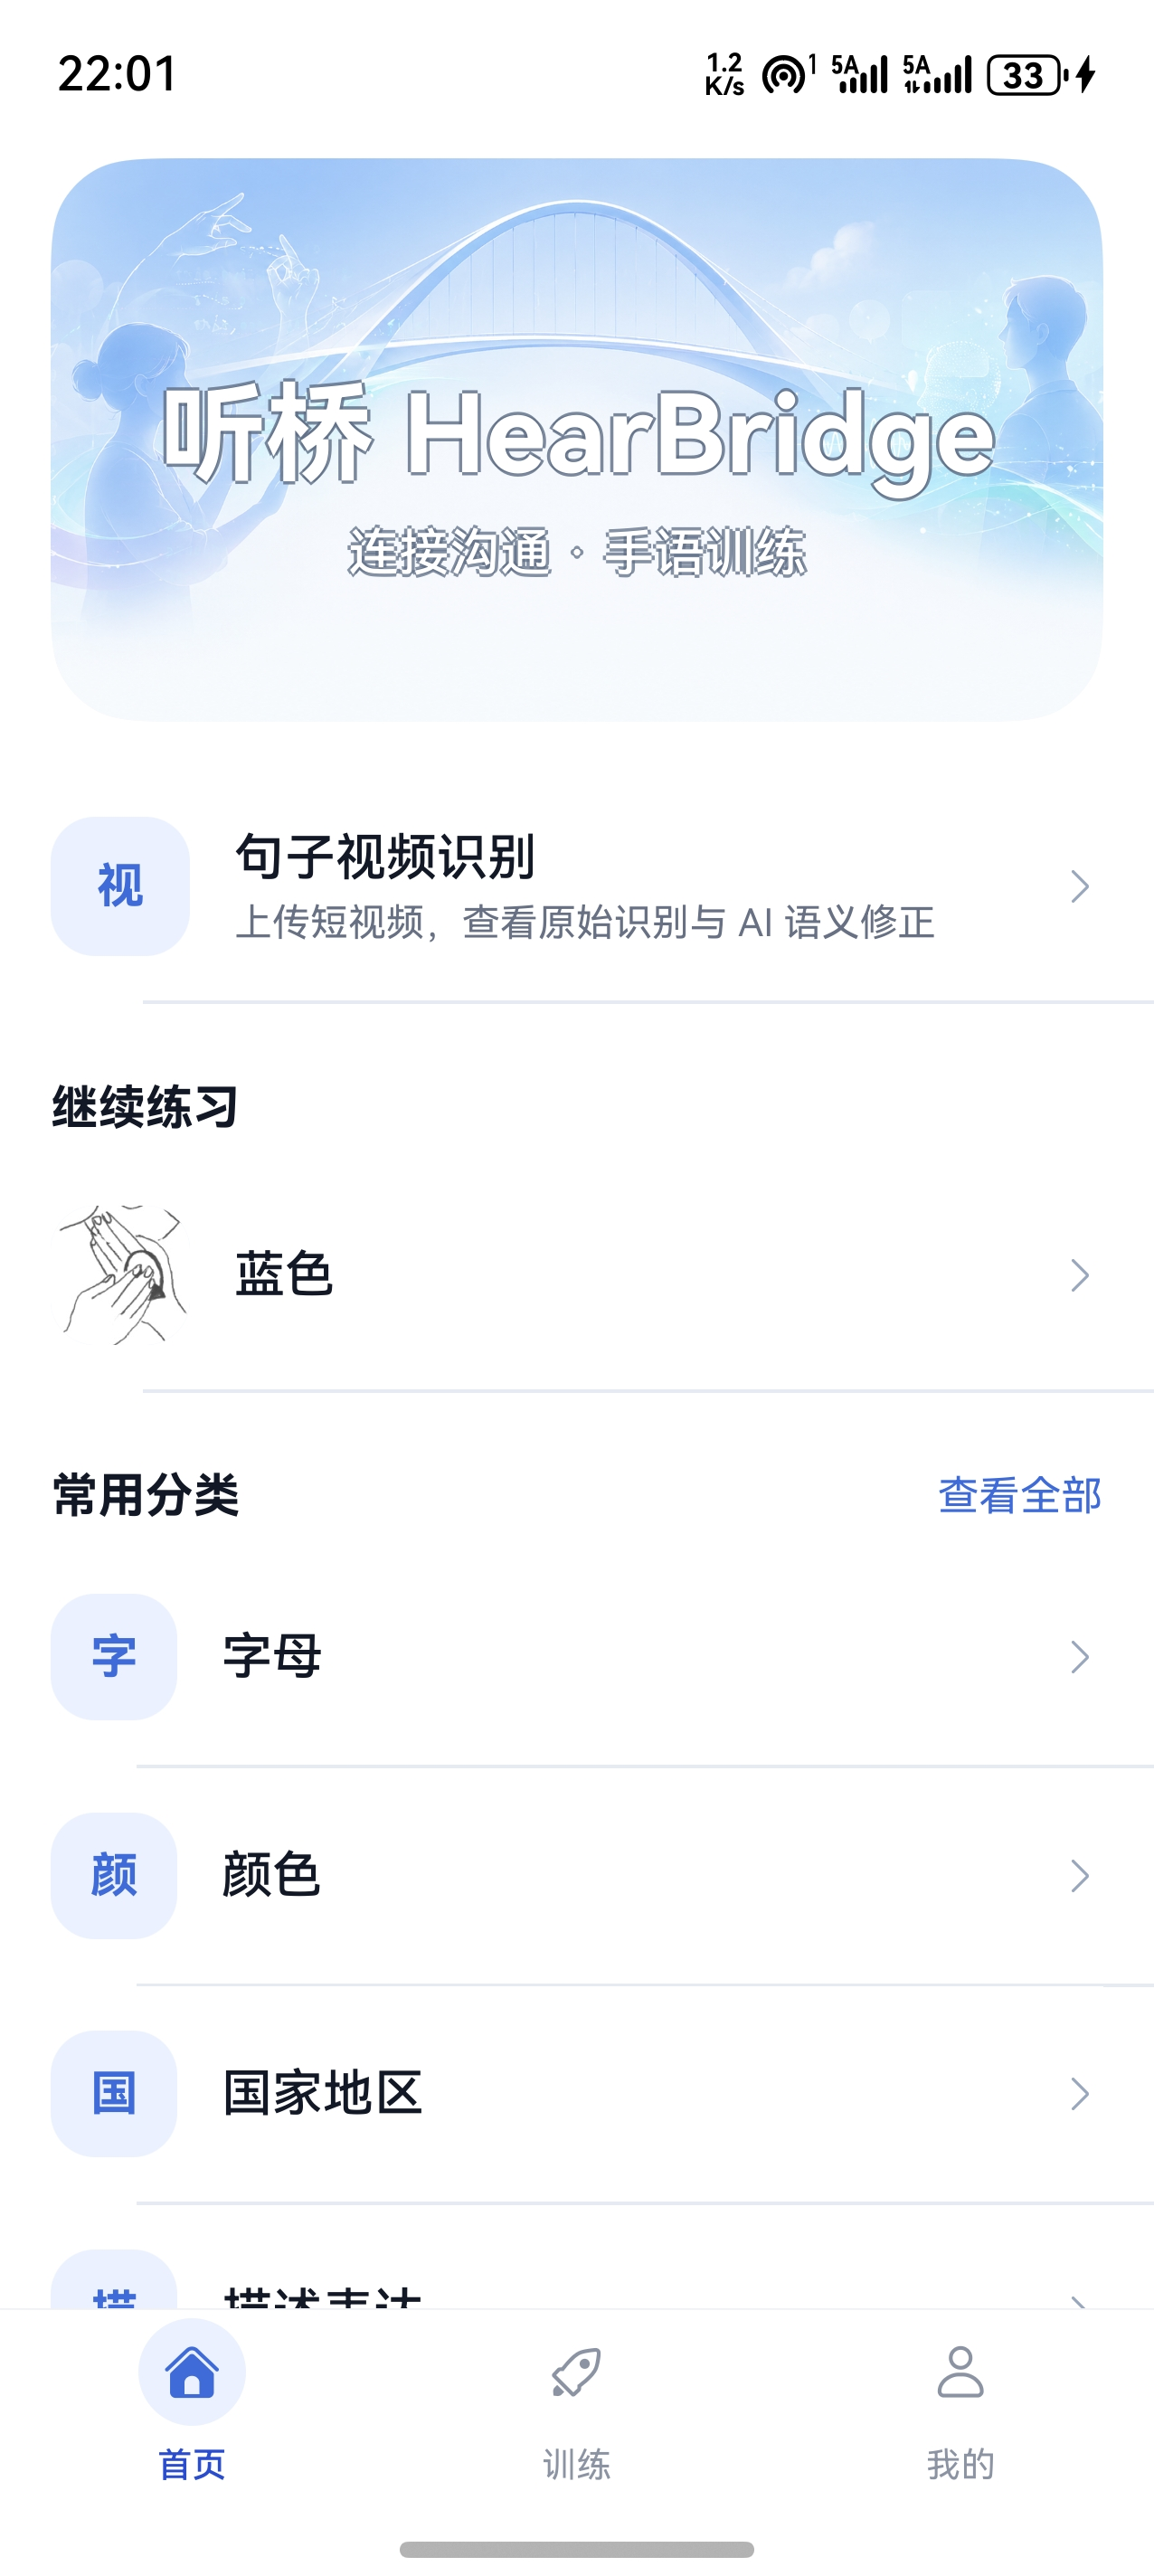
\includegraphics[width=\textwidth,height=0.32\textheight,keepaspectratio]{figures/chapter05/home-page.jpg}
    \caption{首页}
  \end{subfigure}
  \hfill
  \begin{subfigure}[t]{0.235\textwidth}
    \centering
    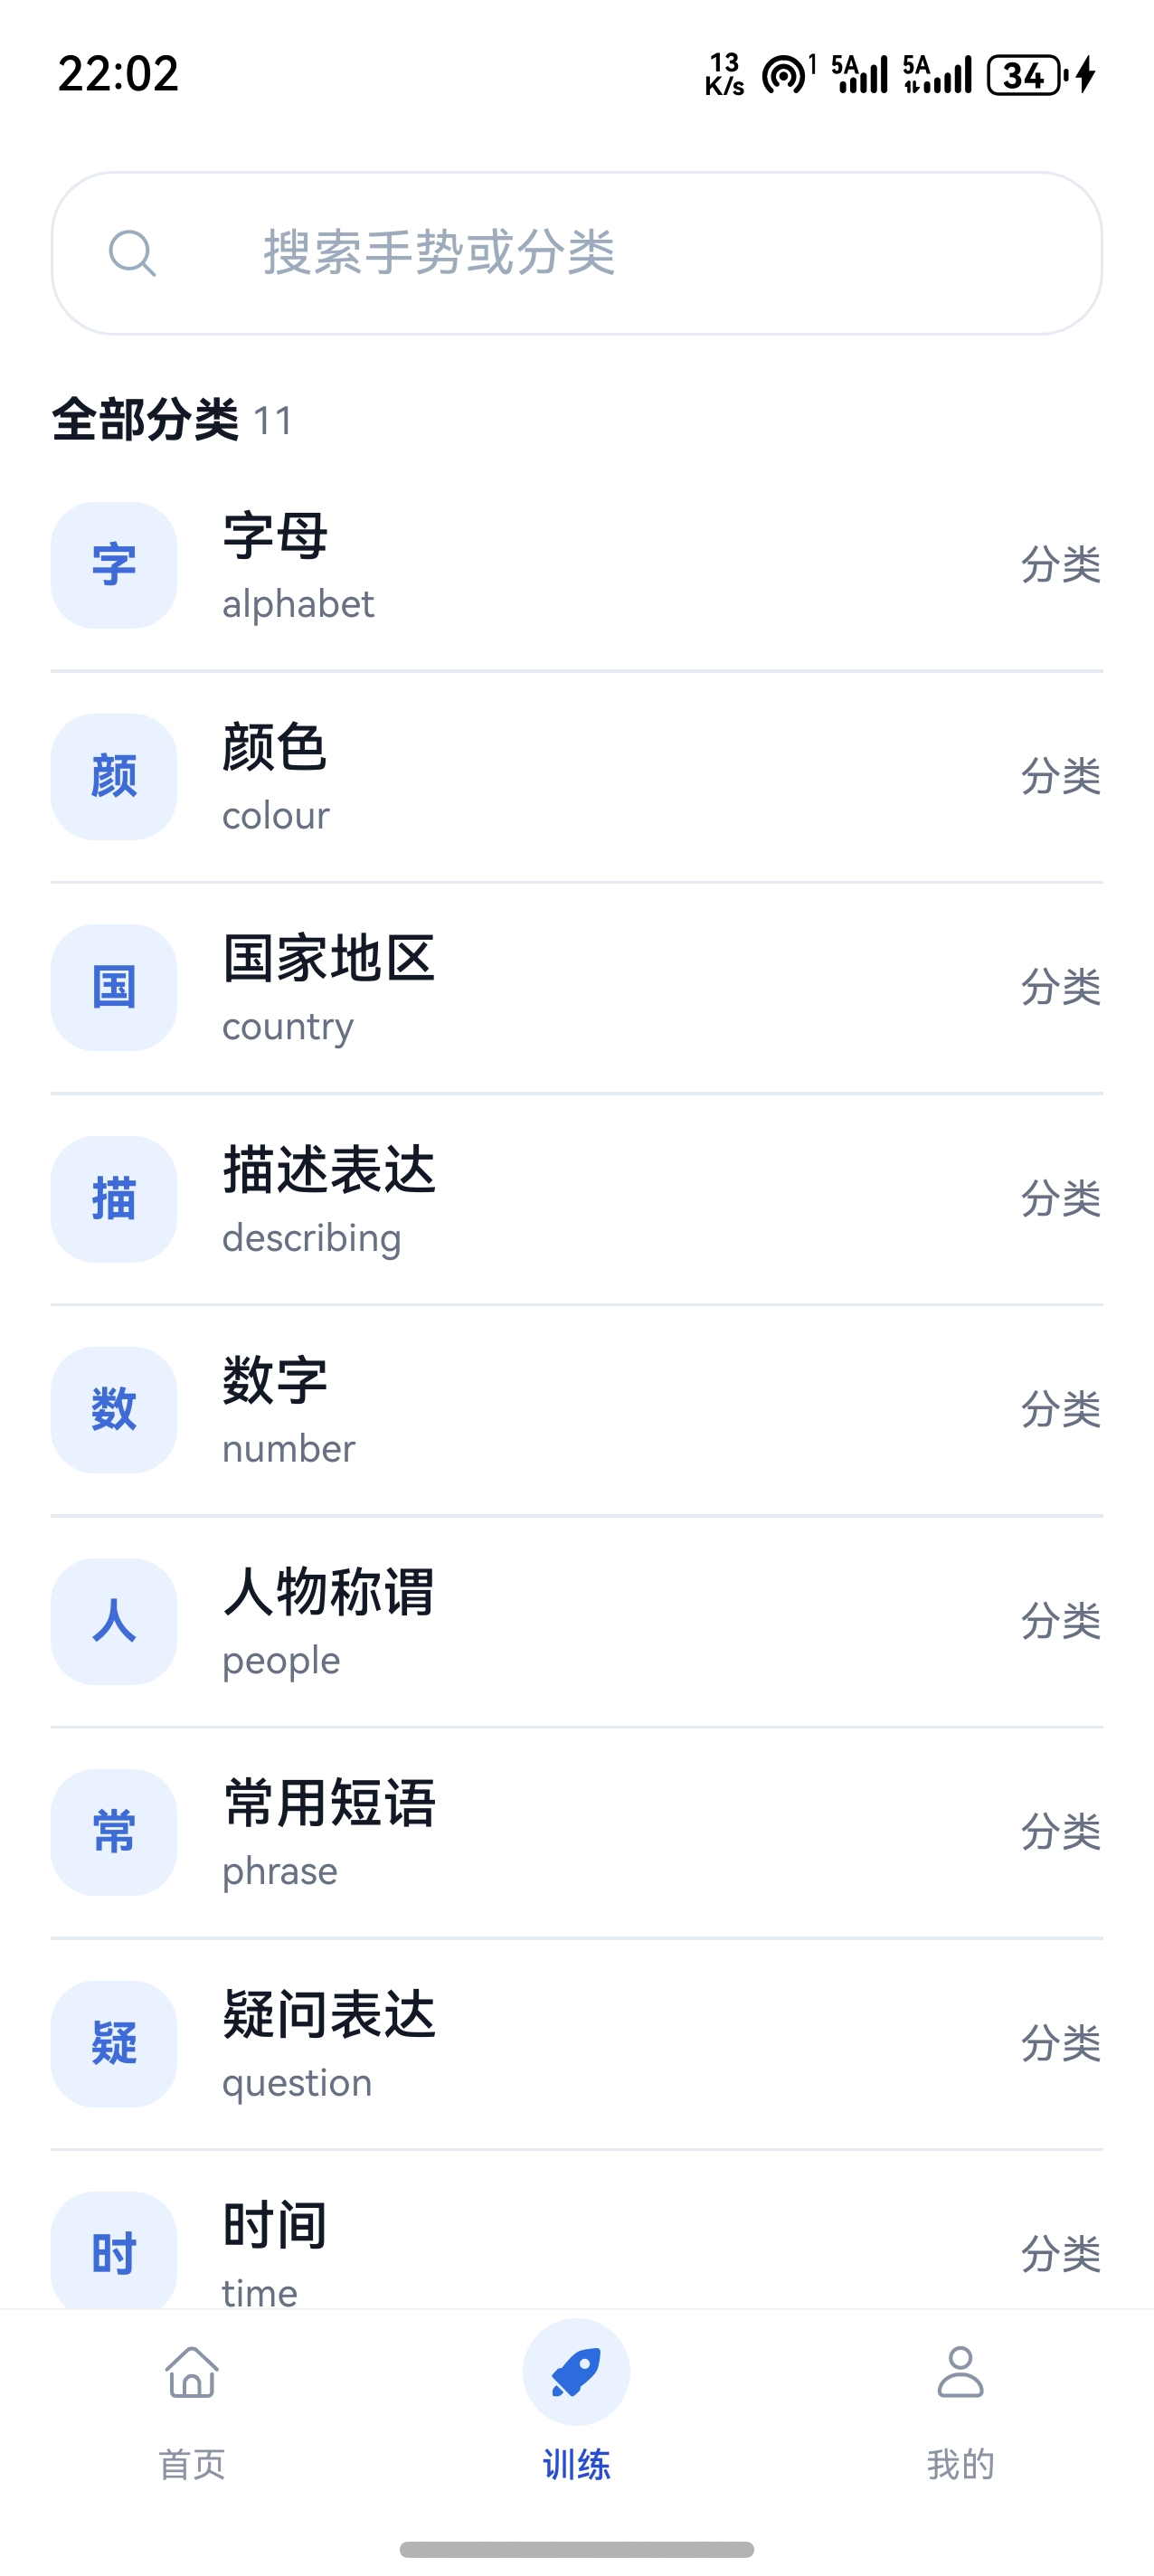
\includegraphics[width=\textwidth,height=0.32\textheight,keepaspectratio]{figures/chapter05/training-page.jpg}
    \caption{训练页}
  \end{subfigure}
  \hfill
  \begin{subfigure}[t]{0.235\textwidth}
    \centering
    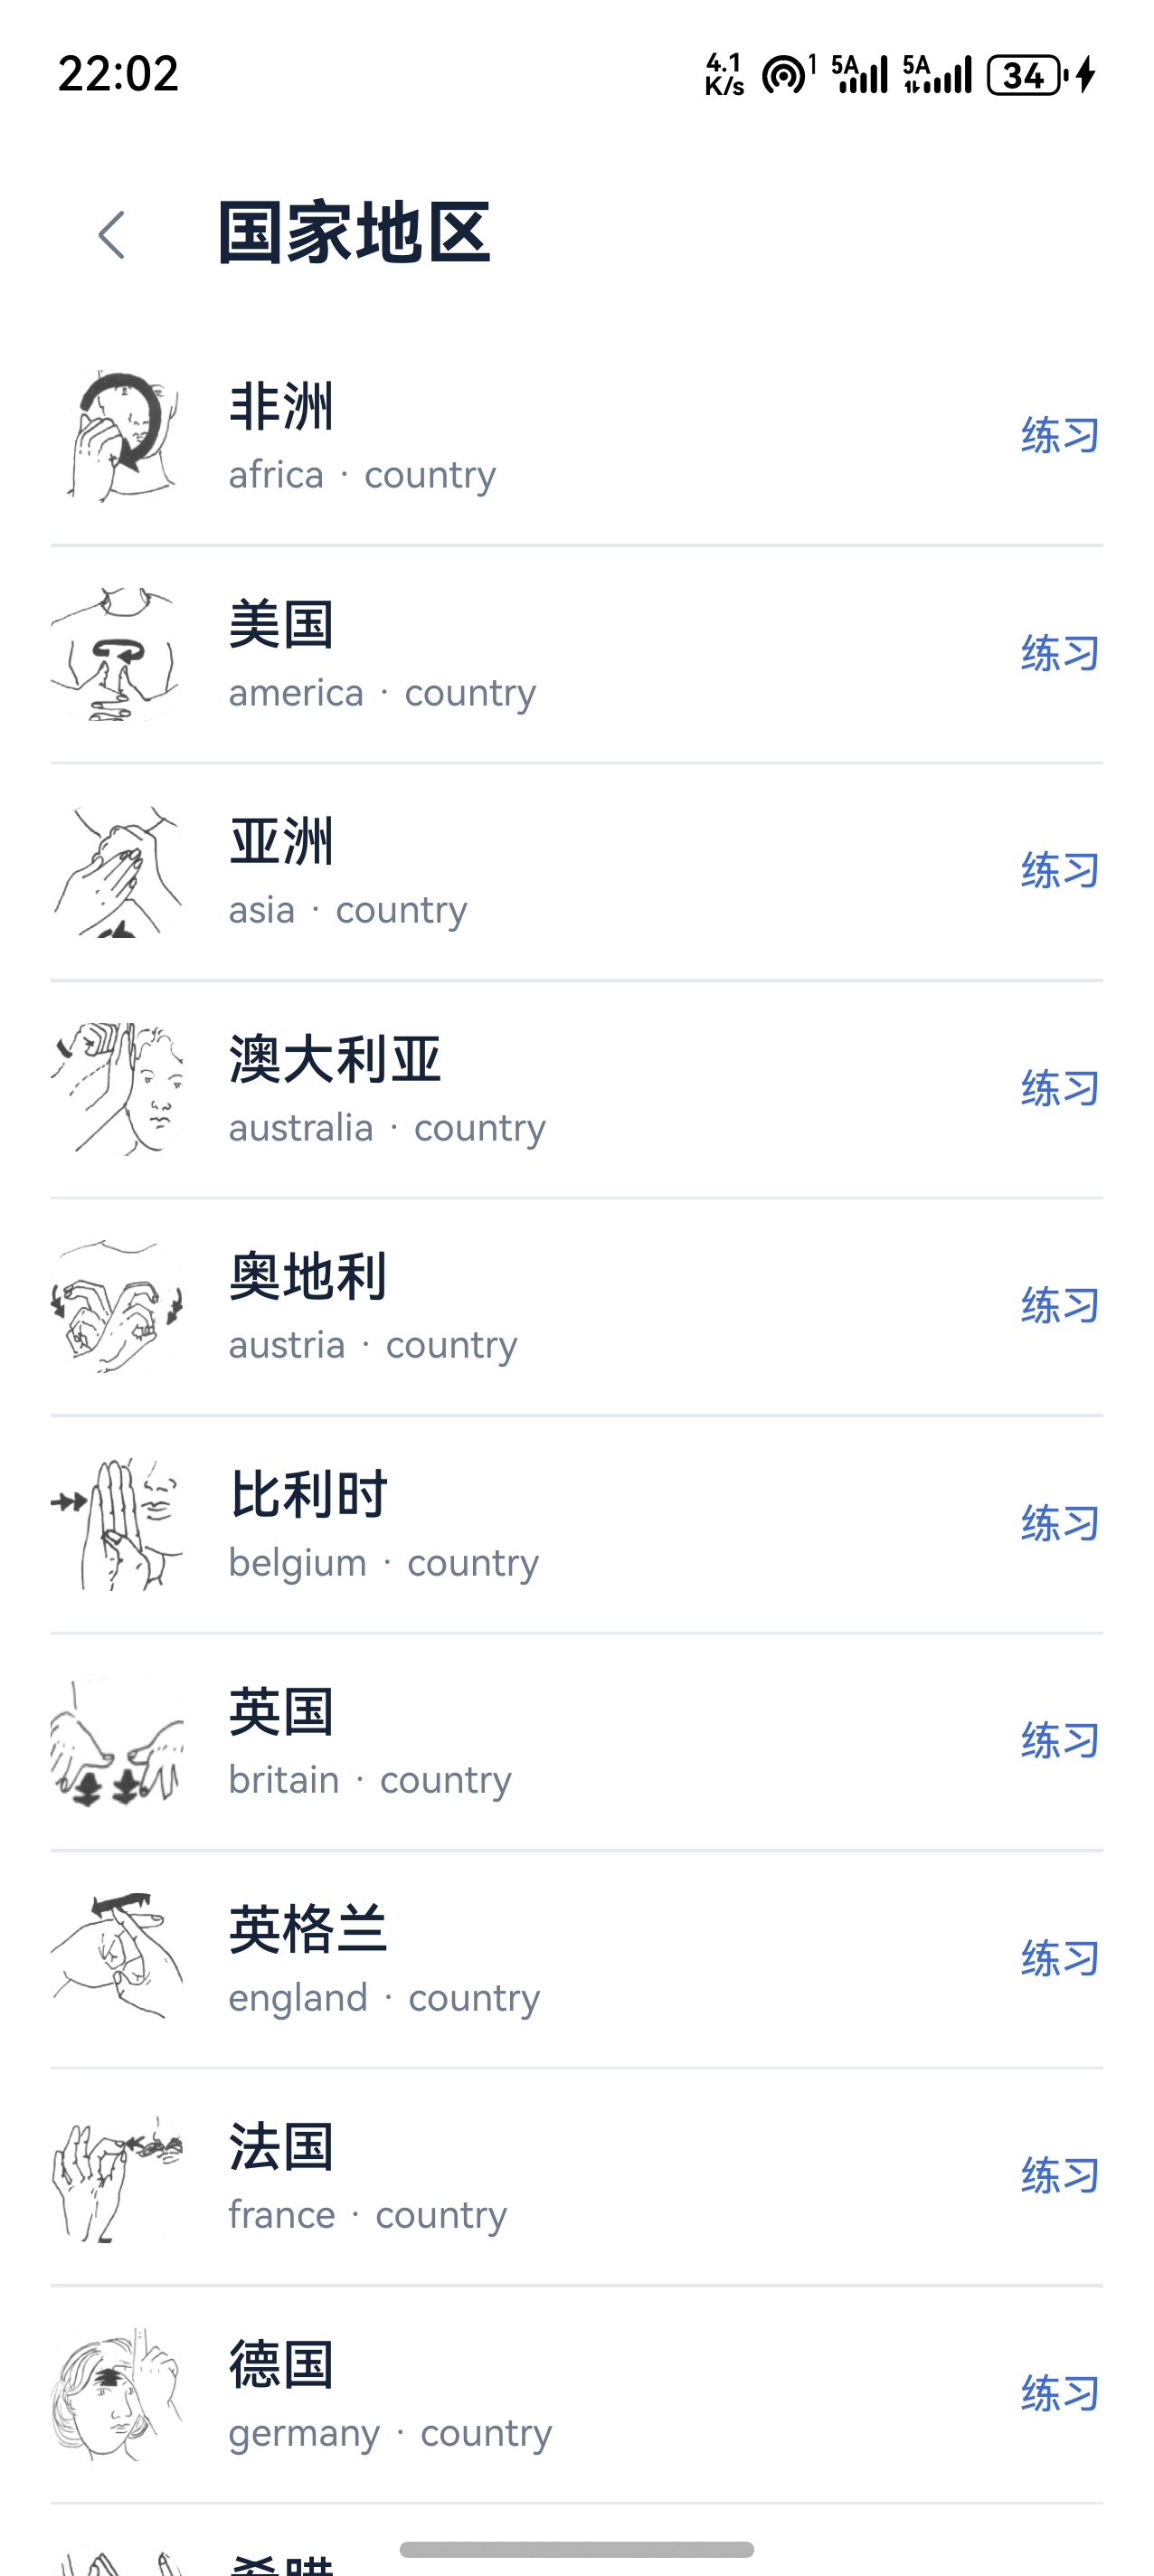
\includegraphics[width=\textwidth,height=0.32\textheight,keepaspectratio]{figures/chapter05/resource-list-page.jpg}
    \caption{资源列表页}
  \end{subfigure}
  \hfill
  \begin{subfigure}[t]{0.235\textwidth}
    \centering
    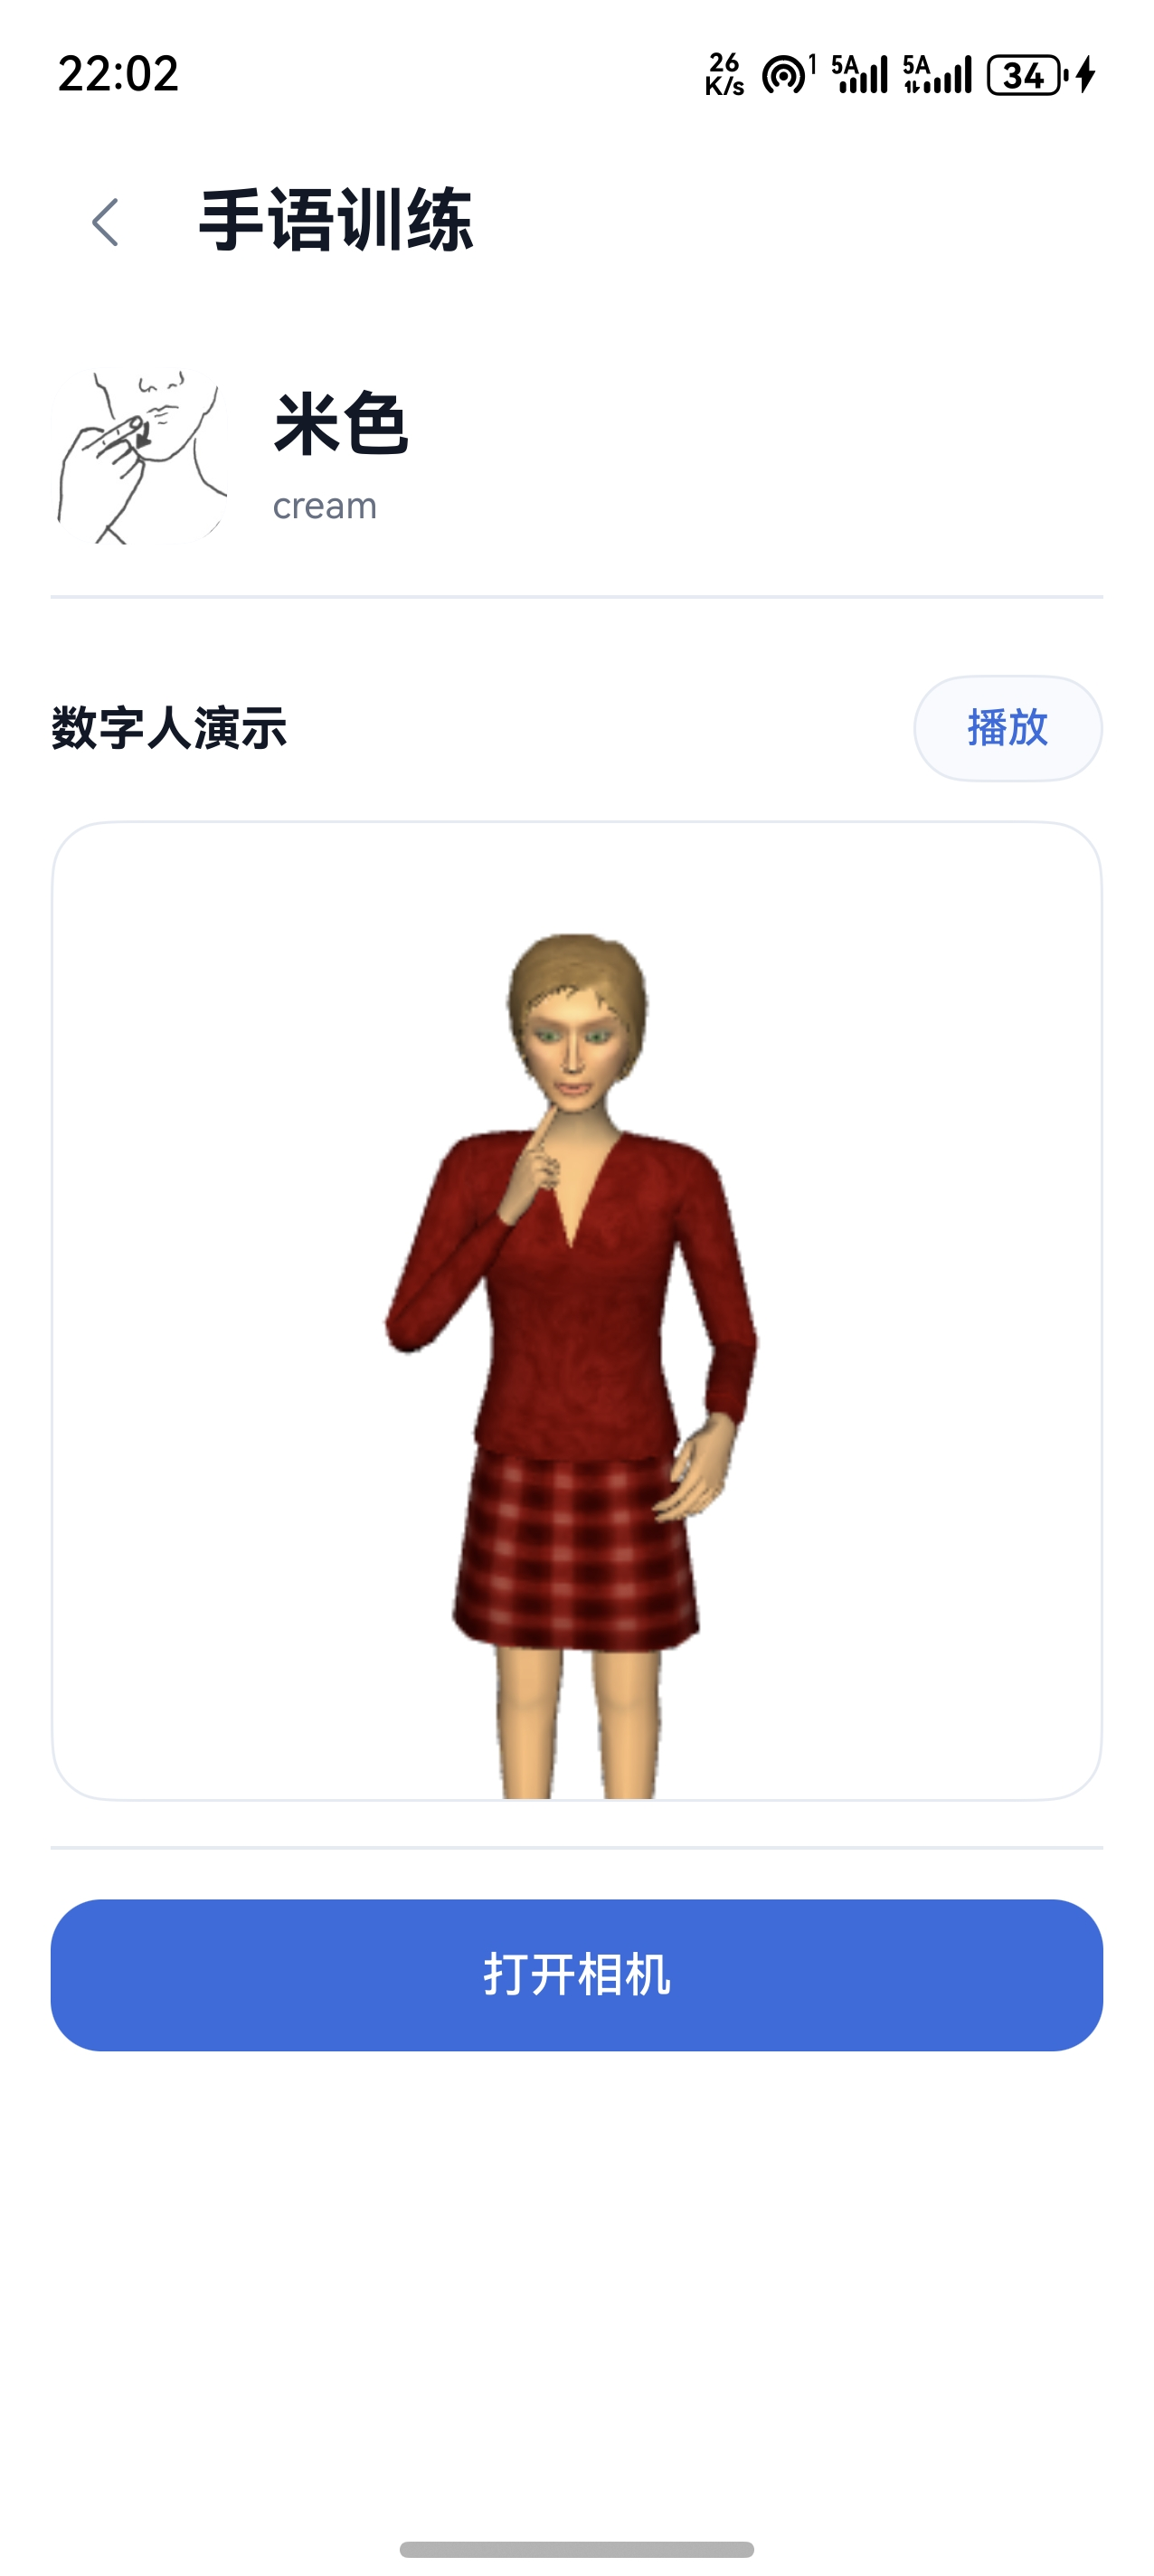
\includegraphics[width=\textwidth,height=0.32\textheight,keepaspectratio]{figures/chapter05/gesture-training-page.jpg}
    \caption{手势训练页}
  \end{subfigure}

  \caption{移动端核心页面效果图}
  \label{fig:chapter05-mobile-core-ui}
\end{figure}

移动端主要调用接口如表~\ref{tab:chapter05-mobile-interfaces} 所示。

\WhuInterfaceTable{移动端主要接口}{tab:chapter05-mobile-interfaces}{
登录认证 & POST & /app/auth/login & 普通用户登录并获取 token \\
用户信息 & GET & /app/user/profile & 获取当前登录用户信息 \\
手势分类 & GET & /app/sign/categories & 获取移动端可见手势分类 \\
手势资源 & GET & /app/sign/resources & 获取可训练手势资源列表 \\
最近练习 & GET & /app/recent-practice & 获取用户最近练习记录 \\
视频识别 & POST & /app/video-recognition & 上传句子视频并获取识别结果 \\
}

\subsection{应用启动、登录恢复与主界面组织实现}

应用启动后首先需要判断用户是否已经登录，并据此决定展示登录注册入口还是进入主界面。
当前移动端入口页面采用登录态驱动的页面切换方式，核心状态由全局登录状态控制。
页面出现时调用初始化逻辑，依次完成登录态恢复、最近练习记录恢复和手语分类加载。

在实现上，应用入口通过 aboutToAppear() 触发 initPage()，再由 restoreAuthState() 恢复本地登录态，由 restoreRecentPracticeFromBackend() 尝试恢复最近练习记录，最后调用 loadCategories() 通过 GestureApi 获取分类数据。
通过这种启动流程，应用能够在用户重新打开时自动恢复登录状态，并尽可能展示最近一次训练相关内容，减少用户重复操作。

主界面采用首页、训练、句子视频识别和个人中心等功能入口组织用户操作路径。
用户登录后，可以从首页查看手语资源和最近练习内容，也可以直接进入训练功能或句子视频识别功能。
个人中心则负责展示用户资料、修改密码和退出登录等操作。
通过这种入口组织方式，移动端将学习、训练、识别和个人管理功能聚合在统一应用内，减少用户在不同功能之间切换时的理解成本。

移动端页面状态主要围绕登录状态、分类列表、最近练习记录、识别结果和用户信息等数据展开。
页面本身不直接承担复杂业务处理，而是通过接口服务和状态管理对象获取数据、更新界面和响应用户操作。
该实现方式符合 HarmonyOS 声明式界面开发特点，也便于后续扩展新的训练入口或识别结果展示形式。

\subsection{手语资源浏览与训练入口实现}

手语资源浏览功能用于向用户展示可学习和训练的手语资源。
移动端在首页或资源页面加载分类数据后，根据分类进一步展示手语资源列表。
用户可以通过资源名称、分类入口或最近练习记录进入具体训练流程。
资源列表中的每一项通常包含资源名称、分类信息、封面或示范资源入口等内容，用于帮助用户快速判断该资源是否为当前需要练习的动作。

在资源浏览实现中，移动端主要通过后端接口获取手势分类和手势资源数据。
分类数据用于构建页面中的分类入口，资源数据则用于构建具体训练项。
由于资源内容由后台管理端维护，移动端不需要在本地写死训练动作，而是根据服务端返回的数据动态展示。
这样，当管理员在后台新增、修改或禁用手势资源后，移动端可以通过接口获取最新资源列表，从而提高系统内容维护的灵活性。

用户选择某个手语资源后，移动端进入训练准备或训练详情页面。
该页面需要展示动作名称、动作说明和标准动作示范入口，并为实时识别训练提供启动按钮。
若资源关联了数字人动作示范或视频资源，移动端可以在训练前展示对应动作，使用户先观察标准动作，再开始模仿训练。
该过程构成了移动端训练功能中的“标准动作展示”阶段。

训练入口的实现重点在于将资源数据、示范资源和识别服务入口连接起来。
用户点击训练按钮后，移动端需要根据当前资源信息构建识别上下文，包括当前训练动作、资源标识和后续结果展示所需的数据。
通过这种方式，移动端能够将资源浏览过程自然过渡到实时训练过程，使用户操作路径从“选择资源”进入“动作练习”。

\subsection{实时手势训练交互实现}

实时手势训练是移动端的核心功能之一。
用户进入训练页面后，应用调用相机采集图像帧，并通过 WebSocket 与 Python 手势识别服务建立实时通信。
移动端持续发送相机图像帧，识别服务返回当前窗口的预测标签、置信度、模型版本等结果，移动端再将识别结果展示给用户。

在实现过程中，移动端需要处理相机权限、相机预览、图像帧获取、WebSocket 连接、识别结果解析和页面状态更新等多个环节。
相机预览用于给用户提供动作调整依据，图像帧发送用于给 Python 识别服务提供输入，识别结果展示则用于形成训练反馈。
为了降低用户等待感，移动端在识别过程中需要及时展示连接状态、识别状态和结果状态，使用户能够判断当前系统是否正在工作。

实时识别结果通常包含预测动作、置信度和模型版本等信息。
移动端接收到结果后，根据当前训练资源和识别结果进行展示。
如果识别结果与当前训练动作一致，可以向用户展示较积极的反馈；
如果识别结果不一致，则可以提示用户调整动作。
当前实现重点并不在移动端完成复杂评分，而是将 Python 识别服务返回的结果组织为用户可理解的训练反馈。

为了保证训练体验，移动端还需要处理识别连接断开、相机帧为空、识别服务异常等情况。
当 WebSocket 连接失败或识别服务不可用时，页面应给出明确提示，而不是让用户停留在无反馈状态。
通过这些状态处理，移动端实时训练功能能够在较复杂的设备和网络环境下保持可用性。

\subsection{句子视频识别页面实现}

除实时单词训练外，移动端还支持句子视频识别功能。
用户可以在移动端选择本地手语句子视频，并提交给服务端进行识别。
服务端接收视频文件后调用 Python 手势识别服务进行视频分析，再结合语义修正服务组织最终结果。
移动端负责展示识别过程状态、原始识别结果、中文映射结果和语义修正结果。

句子视频识别页面效果如图~\ref{fig:chapter05-video-recognition-page} 所示。

\WhuImageFigure[0.42\textwidth][0.68\textheight]{figures/chapter05/video-recognition-page.jpg}{句子视频识别页面效果图}{fig:chapter05-video-recognition-page}

句子视频识别功能的实现过程与实时识别不同。
实时识别强调相机帧的连续传输和即时反馈，而句子视频识别强调视频文件上传、服务端异步处理和结果展示。
移动端在用户选择视频后，需要完成文件选择、上传请求构建、等待识别结果和展示识别结果等步骤。
由于视频识别耗时可能比实时单帧识别更长，页面需要展示加载状态，避免用户误以为操作失败。

识别结果展示时，移动端通常需要区分原始结果和修正结果。
原始结果体现模型识别出的词级序列或候选结果，中文映射结果用于将标签转化为用户可理解的中文词语，语义修正结果则用于展示经过语言组织后的句子表达。
通过分层展示这些结果，用户既可以看到模型的基础识别输出，也可以看到更自然的句子级结果。

该功能体现了移动端与服务端、Python 识别服务和语义修正服务之间的协作关系。
移动端并不直接处理视频识别算法，而是负责将用户输入的视频提交到服务端，并将服务端返回的多层结果转化为清晰的页面展示。
这样可以保持移动端逻辑相对轻量，同时让识别算法和语义处理能力在服务端和识别服务中统一维护。
